Cows are addicted to Assassin's Creed, they start to mock the Leap of Faith -
jumping from Farmer John's aircraft and landing in the haystack in front of their barn!
Because cows are big fan of \t{Game of Thrones}, such behavior is also called Cow's Landing.

\begin{center}
  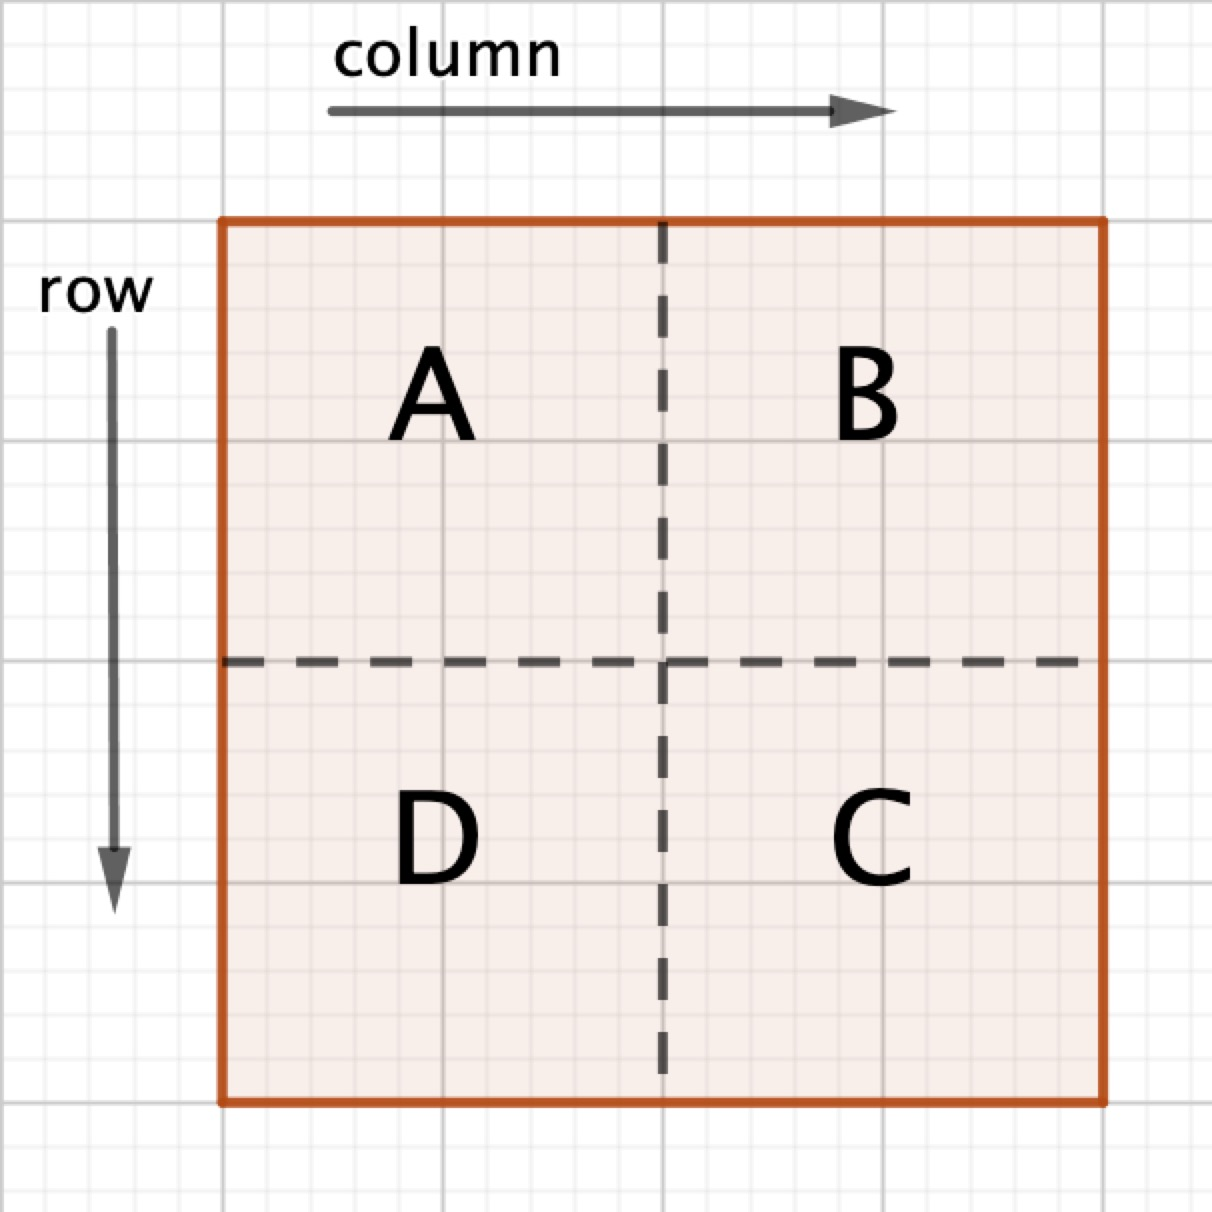
\includegraphics[scale=0.15, natwidth=1212, natheight=1212]{Quat.jpeg}
\end{center}

The farm is in a $2^n$ by $2^n$ grid map, row increases from top to bottom,
column increases from left to right,
and each of cows lives in different barn in a single cell.
One day, cows decide to play Cow's Landing in a special order:

\begin{itemize}
  \item They divided a $2^k$ by $2^k$ grid map into four parts (see the figure above):

  \begin{itemize}
    \item \t{A}: $row \in [1, 2^{k-1}]$, $column \in [1, 2^{k-1})$;
    \item \t{B}: $row \in [1, 2^{k-1}]$, $column \in (2^{k-1}, 2^{k}]$;
    \item \t{C}: $row \in (2^{k-1}, 2^{k}]$, $column \in (2^{k-1}, 2^k]$;
    \item \t{D}: $row \in (2^{k-1}, 2^k]$, $column \in [1, 2^{k-1}]$;
  \end{itemize}

  \item All cows live in \t{A} jump first, then \t{B}, \t{C} and \t{D};
  \item Cows in the smaller region $x$ ($x \in \{A,B,C,D\}$) will apply same ordering recursively.
\end{itemize}

For example, if $n=2$, the total order is:
\begin{table}[h]
  \centering
  \begin{tabular}{|c c c c|}
    \hline
    1   &   2   &   5   &   6   \\
    4   &   3   &   8   &   7   \\
    13  &   14  &   9   &   10  \\
    16  &   15  &   12  &   11  \\
    \hline
  \end{tabular}
\end{table}


Farmer John very cares about his employees, he has prepared $m$ first-aid kits.
Give the rank of a cow in the order, Farmer John needs to know the location of such cow.
